\documentclass[introducao.tex]{subfiles}
\begin{document}
\section{Introdução}
\paragraph{} Este trabalho tem por objetivo o estudo dos fluidos magnéticos. Um algoritmo foi feito para resolver a equação de Navier Stokes em um quadrado unitário. Essa é a equação que governa a dinâmica dos fluidos.

\begin{eqnarray}
\rho\left( \frac{\partial {\textbf{v}}}{\partial t}+\textbf{v}\cdot\nabla \textbf{v} \right)=-\nabla p+\mu\nabla^2 \textbf{v} + \textbf{f}\label{navierstokes}\\
\nabla\cdot\textbf{v}=0
\end{eqnarray}


\subsection{Malha escalonada}
\paragraph{} O algoritmo para resolver a hidrodinâmica foi feito considerando-se uma malha escalonada. Como o magnetismo será acoplado com esse algoritmo, é necessário também utilizar a malha escalonada. $\phi$ será localizada no centro da célula enquanto a força $f$ e os campos $H$ e $B$ estarão normais à celula, como mostrado abaixo. A posição de $H$ e $B$ é a mesma que de $f$.

\begin{center}
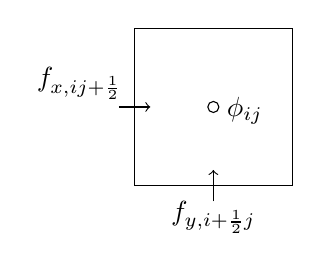
\begin{tikzpicture}
\draw (0,0) rectangle (2,2);
\draw (1.4,0.95) node {$\phi_{ij}$};
\draw[->] (1,-0.2) -- (1,0.2);
\draw (1,-0.4) node {$f_{y,i+\frac{1}{2}j}$};
\draw[->] (-0.2,1) -- (0.2,1);
\draw (-0.7,1.3) node {$f_{x,ij+\frac{1}{2}}$};
\draw (1,1) circle (2pt);
\end{tikzpicture}
\end{center}

\paragraph{} Uma representação de um domínio mais completo está na figura abaixo. Note que cada ponto preto no meio de um bloco é a pressão em ponto interno. Enquanto a pressão em pontos da fronteira imaginária são círculos com interior branco. Pontos na fronteira imaginária são utilizados nos cálculos, mas não precisam ser salvos no resultado final.

\paragraph{} Se é definida, no computador, uma matriz $n\times n$, tem-se $\Delta x = \frac{1}{n-2}$. Os cálculos devem ser todos feitos com base neste $\Delta x$. Além disso, note que as velocidades da extrema esquerda e do extremo inferior não são utilizadas. Você pode declarar tais valores como Not a Number. Se seu programa utilizá-los, há algo errado.

\domainOne

\subsection{Matriz de rotação}
\paragraph{} É útil ter um método de se rotacionar o campo magnético para se testar diferentes configurações do mesmo e analisar simetrias e assimetrias no nosso domínio. Como nosso problema é 2D, tem-se:

\begin{eqnarray}
R(\theta) & =& \left[\begin{array}{cc}
\cos(\theta) & -\sin(\theta)\\
\sin(\theta)  & \cos(\theta)
\end{array}\right]
\end{eqnarray}
\paragraph{} Esta é uma matriz de rotação, logo:
\begin{itemize}
	\item $\det R(\theta) = 1$;
	\item $R^{-1}(\theta) = R^T(\theta)$.
\end{itemize}

\paragraph{} Considere o campo magnético $\mathbf{f}(\mathbf{x})$, no qual $\mathbf{x} = (x,y)$, rotacionado de um ângulo $\theta$. Neste caso, o ponto $\mathbf{x}$ será dado pelo seguinte:

\begin{eqnarray}
\mathbf{f}'(\mathbf{x}) & = & R\cdot \mathbf{f}(R'\cdot \mathbf{x})
\end{eqnarray}

\paragraph{} \textit{Dúvida: se for deslocar o centro do campo magnético, devo fazer isso antes ou depois de rotacionar? Se $\mathbf{f}$ não é linear, fará diferença.}
\end{document}
